\documentclass[journal, a4paper]{IEEEtran}

% some very useful LaTeX packages include:

\usepackage{biblatex}
\addbibresource{cite.bib}


%\usepackage{cite}      % Written by Donald Arseneau
                        % V1.6 and later of IEEEtran pre-defines the format
                        % of the cite.sty package \cite{} output to follow
                        % that of IEEE. Loading the cite package will
                        % result in citation numbers being automatically
                        % sorted and properly "ranged". i.e.,
                        % [1], [9], [2], [7], [5], [6]
                        % (without using cite.sty)
                        % will become:
                        % [1], [2], [5]--[7], [9] (using cite.sty)
                        % cite.sty's \cite will automatically add leading
                        % space, if needed. Use cite.sty's noadjust option
                        % (cite.sty V3.8 and later) if you want to turn this
                        % off. cite.sty is already installed on most LaTeX
                        % systems. The latest version can be obtained at:
                        % http://www.ctan.org/tex-archive/macros/latex/contrib/supported/cite/

\usepackage{graphicx}   % Written by David Carlisle and Sebastian Rahtz
                        % Required if you want graphics, photos, etc.
                        % graphicx.sty is already installed on most LaTeX
                        % systems. The latest version and documentation can
                        % be obtained at:
                        % http://www.ctan.org/tex-archive/macros/latex/required/graphics/
                        % Another good source of documentation is "Using
                        % Imported Graphics in LaTeX2e" by Keith Reckdahl
                        % which can be found as esplatex.ps and epslatex.pdf
                        % at: http://www.ctan.org/tex-archive/info/

%\usepackage{psfrag}    % Written by Craig Barratt, Michael C. Grant,
                        % and David Carlisle
                        % This package allows you to substitute LaTeX
                        % commands for text in imported EPS graphic files.
                        % In this way, LaTeX symbols can be placed into
                        % graphics that have been generated by other
                        % applications. You must use latex->dvips->ps2pdf
                        % workflow (not direct pdf output from pdflatex) if
                        % you wish to use this capability because it works
                        % via some PostScript tricks. Alternatively, the
                        % graphics could be processed as separate files via
                        % psfrag and dvips, then converted to PDF for
                        % inclusion in the main file which uses pdflatex.
                        % Docs are in "The PSfrag System" by Michael C. Grant
                        % and David Carlisle. There is also some information
                        % about using psfrag in "Using Imported Graphics in
                        % LaTeX2e" by Keith Reckdahl which documents the
                        % graphicx package (see above). The psfrag package
                        % and documentation can be obtained at:
                        % http://www.ctan.org/tex-archive/macros/latex/contrib/supported/psfrag/

%\usepackage{subfigure} % Written by Steven Douglas Cochran
                        % This package makes it easy to put subfigures
                        % in your figures. i.e., "figure 1a and 1b"
                        % Docs are in "Using Imported Graphics in LaTeX2e"
                        % by Keith Reckdahl which also documents the graphicx
                        % package (see above). subfigure.sty is already
                        % installed on most LaTeX systems. The latest version
                        % and documentation can be obtained at:
                        % http://www.ctan.org/tex-archive/macros/latex/contrib/supported/subfigure/

\usepackage{url}        % Written by Donald Arseneau
                        % Provides better support for handling and breaking
                        % URLs. url.sty is already installed on most LaTeX
                        % systems. The latest version can be obtained at:
                        % http://www.ctan.org/tex-archive/macros/latex/contrib/other/misc/
                        % Read the url.sty source comments for usage information.

%\usepackage{stfloats}  % Written by Sigitas Tolusis
                        % Gives LaTeX2e the ability to do double column
                        % floats at the bottom of the page as well as the top.
                        % (e.g., "\begin{figure*}[!b]" is not normally
                        % possible in LaTeX2e). This is an invasive package
                        % which rewrites many portions of the LaTeX2e output
                        % routines. It may not work with other packages that
                        % modify the LaTeX2e output routine and/or with other
                        % versions of LaTeX. The latest version and
                        % documentation can be obtained at:
                        % http://www.ctan.org/tex-archive/macros/latex/contrib/supported/sttools/
                        % Documentation is contained in the stfloats.sty
                        % comments as well as in the presfull.pdf file.
                        % Do not use the stfloats baselinefloat ability as
                        % IEEE does not allow \baselineskip to stretch.
                        % Authors submitting work to the IEEE should note
                        % that IEEE rarely uses double column equations and
                        % that authors should try to avoid such use.
                        % Do not be tempted to use the cuted.sty or
                        % midfloat.sty package (by the same author) as IEEE
                        % does not format its papers in such ways.

\usepackage{amsmath}    % From the American Mathematical Society
                        % A popular package that provides many helpful commands
                        % for dealing with mathematics. Note that the AMSmath
                        % package sets \interdisplaylinepenalty to 10000 thus
                        % preventing page breaks from occurring within multiline
                        % equations. Use:
%\interdisplaylinepenalty=2500
                        % after loading amsmath to restore such page breaks
                        % as IEEEtran.cls normally does. amsmath.sty is already
                        % installed on most LaTeX systems. The latest version
                        % and documentation can be obtained at:
                        % http://www.ctan.org/tex-archive/macros/latex/required/amslatex/math/



% Other popular packages for formatting tables and equations include:

%\usepackage{array}
% Frank Mittelbach's and David Carlisle's array.sty which improves the
% LaTeX2e array and tabular environments to provide better appearances and
% additional user controls. array.sty is already installed on most systems.
% The latest version and documentation can be obtained at:
% http://www.ctan.org/tex-archive/macros/latex/required/tools/

% V1.6 of IEEEtran contains the IEEEeqnarray family of commands that can
% be used to generate multiline equations as well as matrices, tables, etc.

% Also of notable interest:
% Scott Pakin's eqparbox package for creating (automatically sized) equal
% width boxes. Available:
% http://www.ctan.org/tex-archive/macros/latex/contrib/supported/eqparbox/

% *** Do not adjust lengths that control margins, column widths, etc. ***
% *** Do not use packages that alter fonts (such as pslatex).         ***
% There should be no need to do such things with IEEEtran.cls V1.6 and later.


% Your document starts here!
\begin{document}
\begin{titlepage}

\newcommand{\HRule}{\rule{\linewidth}{0.5mm}} % Defines a new command for the horizontal lines, change thickness here

\center % Center everything on the page
 %----------------------------------------------------------------------------------------
%	LOGO SECTION
%----------------------------------------------------------------------------------------

~\\[1cm]

\includegraphics{SCUT.png}\\[2cm] % Include a department/university logo - this will require the graphicx package

%----------------------------------------------------------------------------------------
%	TITLE SECTION
%----------------------------------------------------------------------------------------

\HRule \\[1cm]
{ \huge \bfseries The Experiment II Report of \textit{Machine Learning} }\\[0.6cm] % Title of your document
\HRule \\[2cm]
%----------------------------------------------------------------------------------------
%	HEADING SECTIONS
%----------------------------------------------------------------------------------------


\textsc{\LARGE \textbf{School:} School of Software Engineering}\\[1cm]
\textsc{\LARGE \textbf{Subject:} Software Engineering}\\[2cm] 

 
%----------------------------------------------------------------------------------------
%	AUTHOR SECTION
%----------------------------------------------------------------------------------------

\begin{minipage}{0.4\textwidth}
\begin{flushleft} \large
\emph{Author:}\\
Jianqiao Hu % Your name
\end{flushleft}
\end{minipage}
~
\begin{minipage}{0.4\textwidth}
\begin{flushright} \large
\emph{Supervisor:} \\
Qingyao Wu
\end{flushright}
\end{minipage}\\[2cm]
~
\begin{minipage}{0.4\textwidth}
\begin{flushleft} \large
\emph{Student ID:}\\
202221045886
\end{flushleft}
\end{minipage}
~
\begin{minipage}{0.4\textwidth}
\begin{flushright} \large
\emph{Grade:} \\
Graduate
\end{flushright}
\end{minipage}\\[2cm]

% If you don't want a supervisor, uncomment the two lines below and remove the section above
%\Large \emph{Author:}\\
%John \textsc{Smith}\\[3cm] % Your name

%----------------------------------------------------------------------------------------
%	DATE SECTION
%----------------------------------------------------------------------------------------

{\large \today}\\[2cm] % Date, change the \today to a set date if you want to be precise

 
%----------------------------------------------------------------------------------------

\vfill % Fill the rest of the page with whitespace

\end{titlepage}


% Define document title and author
	\title{English-Chinese Translation Machine Based on Sequence to Sequence Network}
	\author{Jianqiao Hu \thanks{autor's email: 202221045886@mail.scut.edu.cn}}
	\maketitle

% Write abstract here
\begin{abstract}
This report is about second experience in machine learning. We explained how to build a anaconda environment to launch python scripts to train a model in machine translation. In second part, we have pre-processed raw training data and trained a Encoder-Decoder model to translate English into Chinese. Consequently, statistics of this experience was been attached.
\end{abstract}

% Each section begins with a \section{title} command
\section{Introduction}
	% \PARstart{}{} creates a tall first letter for this first paragraph
\PARstart{L}{anguages} are carriers of information transmission. Many kinds of languages are being using among whole world. One of research target in natural language processing field is how translate a language into another language accurately. With the inspiration from classic sequence-to-sequence machine translation models like \cite{1703.01619} and attention mechanism added machine learning language translation models like \cite{10.5555/3295222.3295349}. The first time that Encoder-Decoder likes model used in machine translation was \cite{cho-etal-2014-learning}. In this method, Gated Recurrent Unit (GRU) was added into model to catch history information between tokens. Another literature whose proposes model used Encoder-Decoder model to translate natural languages is \cite{10.5555/2969033.2969173} while it used Long Short Term Memory (LSTM) to learn implicit connection information from sequence.

% Main Part
\section{Methods and Theory}
In this experience, its algorithm elaborates an encoder-decoder model with attention mechanism and conditional possibility in machine translation. In this algorithm, it defined a sentence like $ Y=[y_1,y_2,...,y_{t}] $. In this case, conditional probability distribution $ p(Y) $ in sequence Y is equation.\ref{probability} while T is the length of whole sentence and $ c  $ is the semantic vector calculated from each hidden state form a sentence in equation.\ref{sv}.

\begin{equation}
    p(Y)= \prod_{t=1}^{T} \label{probability}p(y_t|y_1,y_2,...,y_{t},c)
\end{equation}

\begin{equation}
    c=q([h_1,h_2,...,h_T]) \label{sv}
\end{equation}

For attention mechanism this algorithm used contributes a hidden state in procession of machine learning for a neural cell to another like equation.\ref{hidden} while $ f(\cdot) $ is the function to calculate hidden state from $ x_t $ and $ h_{t-1} $.

\begin{equation}
    h_t=f(x_t,h_{t-1}) \label{hidden}
\end{equation}




\section{Experiments}
\subsection{Dataset}
In this experience, we used English-Chinese translation dataset to train the model. In this case, this experience's model can convert English to Chinese and convert Chinese to English. Each pair of translation data is on the same format: English sentence is in the left, Chinese sentence is in the middle position, and other attribute information in the right.

\subsection{Result}

In training processing, the input sentence is passed to the encoder and each output and the final hidden state are recorded. The $ <SOS> $ (which means "start of sentence") token is fed as the first input to the decoder and the final hidden state of the encoder as its first hidden state.
We use BLEU from \cite{papineni-etal-2002-bleu} to reveal the effect of this translation model.

Because in this experience, we didn't split out test dataset and training dataset, in final, the BLEU score of this model is almost approach to 1, which illustrates that translation result is similar to the training dataset. BLEU score of experience result is Fig.\ref{fig:bleu}. In this image, models selected some sentence written by English from dataset randomly. It shows that sentence was been translated into Chinese exactly by model. For example, in Fig.\ref{fig:bleu}, a sentence is "she is sitting on the bench ." in English was translated into Chinese as truly meaning and $ <EOS> $ means "end of sentence".

Training loss in this experience was a little discrepancy in between difference of maximum number of tokens in a sentence. For example, we attach two pictures which reflect the change of loss value in two different maximum number of tokens in a sentence like Fig.\ref{fig:loss1} with maximum of 20 while Fig.\ref{fig:loss2} with maximum of 15 in this experience. 


\section{Conclusion}
	This experience addresses the question that whether attention mechanism could excavate deep information between tokens in sentence deeply. In this experience, we trains a model to translate English sentences into Chinese one. This model use encoder-decoder likes architecture to grab implication of English sentences from sentence vectors in hidden state.
	
	\begin{figure}
		% Center the figure.
		\begin{center}
		% Include the eps file, scale it such that it's width equals the column width. You can also put width=8cm for example...
		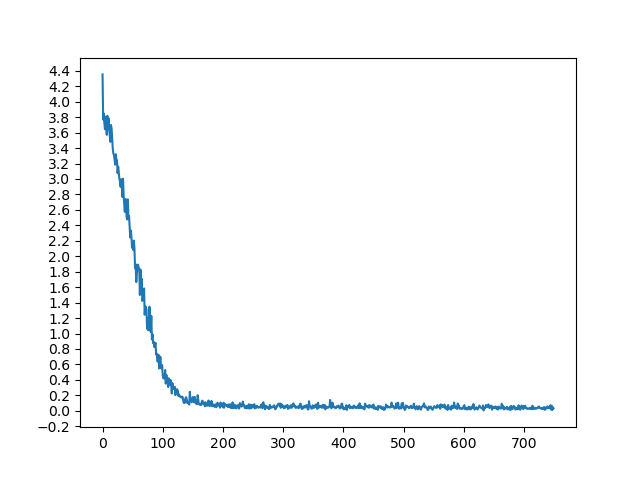
\includegraphics[width=\columnwidth]{images/loss1.png}
		% Create a subtitle for the figure.
		\caption{loss in maximum number of 20}
		% Define the label of the figure. It's good to use 'fig:title', so you know that the label belongs to a figure.
		\label{fig:loss1}
		\end{center}
	\end{figure}
	
		\begin{figure}
		% Center the figure.
		\begin{center}
		% Include the eps file, scale it such that it's width equals the column width. You can also put width=8cm for example...
		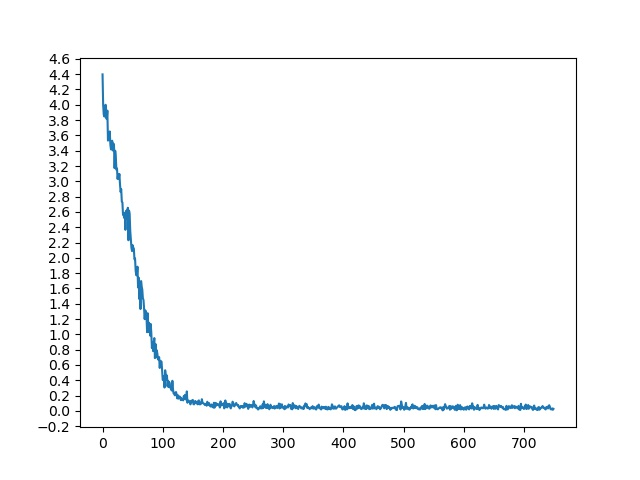
\includegraphics[width=\columnwidth]{images/loss2.jpg}
		% Create a subtitle for the figure.
		\caption{loss in maximum number of 15}
		% Define the label of the figure. It's good to use 'fig:title', so you know that the label belongs to a figure.
		\label{fig:loss2}
		\end{center}
	\end{figure}
	
		\begin{figure}
		% Center the figure.
		\begin{center}
		% Include the eps file, scale it such that it's width equals the column width. You can also put width=8cm for example...
		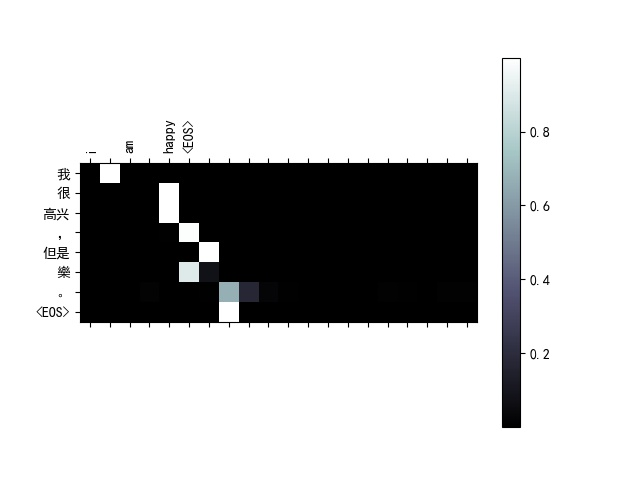
\includegraphics[width=\columnwidth]{images/result-i am happy.jpg}
		% Create a subtitle for the figure.
		\caption{result of translate}
		% Define the label of the figure. It's good to use 'fig:title', so you know that the label belongs to a figure.
		\label{fig:result1}
		\end{center}
	\end{figure}
	
	\begin{figure}
		% Center the figure.
		\begin{center}
		% Include the eps file, scale it such that it's width equals the column width. You can also put width=8cm for example...
		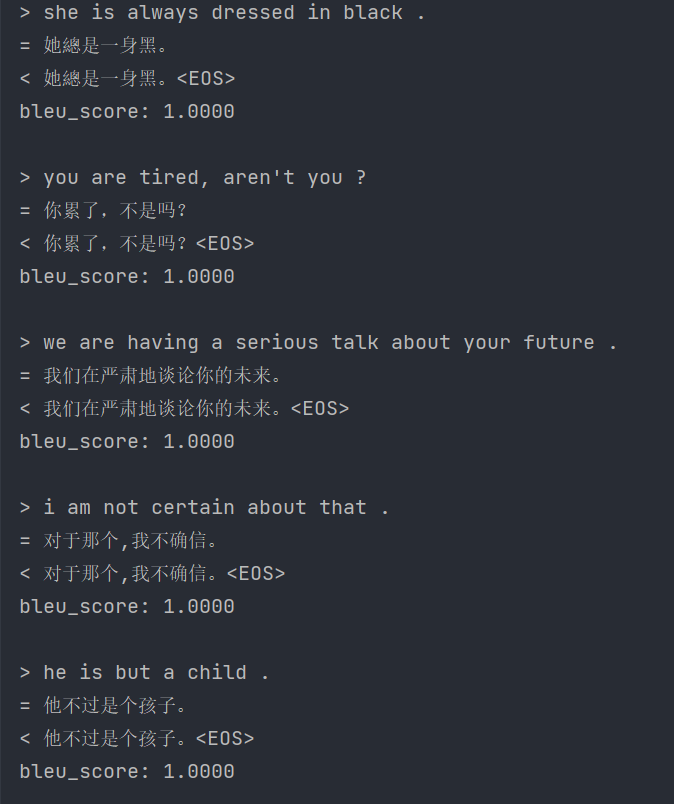
\includegraphics[width=\columnwidth]{images/bleu.png}
		% Create a subtitle for the figure.
		\caption{BLEU score of test}
		% Define the label of the figure. It's good to use 'fig:title', so you know that the label belongs to a figure.
		\label{fig:bleu}
		\end{center}
	\end{figure}
	
	

\printbibliography

% Your document ends here!
\end{document}

